\section{Integration }

In order to approximate the pressure on either side of the airfoil, an integral computation algorithm needs to be implemented.
Three different computation methods were considered, the goal being to find the algorithm with the highest convergence speed.


\subsection{Trapezoidal Method}

The trapezoidal method approximates the area under the curve of the function by dividing it into trapezoids and summing their areas.

Considering $n$ as the number of trapezoids used, the algorithm's time complexity is $\mathcal{O}(n)$.
By increasing $n$, the result's accuracy is improved, but the execution time is longer.

Despite its simplicity, the level of accuracy given by this method is very good for performing simple computations.


\subsection{Simpson's Rule}

Simpson's rule gives a second-order approximation of the integral of $f$ over $[a, b]$,
which means that the result is approximated using a parabola instead of a straight line, as in the previous method.
Its implementation uses an approximation similar to the one used in the previous method (see equation~\ref{eq:simpson-rule}).

\begin{equation}
	\label{eq:simpson-rule}
	\int_{x_i}^{x_{i + 1}} f(x) dx \approx \frac{x_{i + 1} - x_i}{3} \left[ f(x_i) + 4 \times f\left(\frac{x_i + x_{i + 1}}{2}\right) + f(x_{i + 1}) \right]
\end{equation}

Given this approximation, the integral of the function $f$ can be approximated by summing these results over all the sub-intervals,
$[x_i, x_{i + 1}]$ in $[a, b]$, as shown in equation~\ref{eq:simpson-rule-sum}.

\begin{equation}
	\label{eq:simpson-rule-sum}
	\int_a^b f(x) dx \approx \sum_{i = 0}^{n - 1} \int_{x_i}^{x_{i + 1}} f(x) dx
\end{equation}

As a result, this method's time complexity is $\mathcal{O}(n)$, where $n$ is the number of sub-intervals.


\subsection{Romberg's Method}

Romberg's method gives a more accurate approximation of the integral of $f$ over $[a, b]$ than the previous ones.
This method fills a table with the results of the trapezoidal method (first column), with a given number of evaluations.
The results of the previous rows are then used to compute the next rows, 
using both equations~\ref{eq:romberg-method-init} and~\ref{eq:romberg-method}.

It can be noted that the different rows represent integration methods using polynomials of increasing order.
Thus, this method generalizes the ones that were implemented before, considering both previous methods are special cases of this one, mathematically speaking.

\begin{equation}
	\label{eq:romberg-method-init}
	R_{n, 0} = h_n \times \left(\frac{f(a) + f(b)}{2} + \sum_{k = 0}^{2^{n - 1} - 1} f(x_k)\right)
	\text{where}\ h_n = \frac{b - a}{2^n}\ \text{and}\ x_k = a + k \times h_n
\end{equation}

\begin{equation}
	\label{eq:romberg-method}
	R_{n, m} = \frac{4^m R_{n, m - 1} - R_{n - 1, m - 1}}{4^m - 1}\ \text{where}\ n, m > 0
\end{equation}

In order to fill the table in the correct order, the columns must be filled from left to right, and the rows from top to bottom.
Once the table is filled, the result of the integral is the bottom right element of the table.

Another point to consider is that this method requires fewer evaluations on the function than the previous ones, given that evaluations are reused for the other columns.
Thus, when dealing with complex functions, this method is more efficient than the previous ones.

This method's time complexity depends on the table's size. In terms of memory, a 2-dimensional array is required. As a result, the memory complexity is $\mathcal{O}(n^2)$, where $n$ is the number of rows,
which means that this method requires more memory access, and thus slower.


\subsection{Integration with a Given Precision}

The following method offers the possibility of computing the integral of a function with a specific precision.
Its implementation uses the same algorithm from Romberg's method, except that it stops when the algorithm reaches the expected precision.

In fact, the algorithm stops when the equation $\left| R_{n, m} - R_{n - 1, m - 1} \right| \leq \epsilon$ is satisfied,
i.e. when the difference between the current result and the previous one is less than the given precision.

This method seemed to be the longest to apply, but is the most accurate among all the methods that were implemented, given that the precision can be chosen, which is essential for some applications.


\subsection{Comparison of Convergence Speeds}

The convergence speed of each method is displayed in Figure~\ref{fig:convergence}.

\medbreak

The trapezoidal method has a linear convergence rate, which means that the error decreases at a rate proportional to $1/n$, where $n$ is the number of sub-intervals.
This rate of convergence is not very fast, but it is generally sufficient for most applications.

\smallbreak
Simpson's rule has a faster convergence rate than the trapezoidal method, which is proportional to $1/n^2$.
This means that it typically requires fewer sub-intervals to achieve a given level of accuracy compared to the trapezoidal method. However, it can be sensitive to the shape of the function being integrated, and may not always be applicable.

\smallbreak
Romberg's method has a much faster convergence rate than both the trapezoidal method and Simpson's rule.
Its convergence rate is exponential, which means that the error decreases at a rate proportional to $2^{-2m}$, where $m$ is the number of iterations.
This means that it can achieve a high accuracy level with relatively few function evaluations, making it very efficient for many applications.
However, it requires more memory to store intermediate results, and can be more computationally intensive in some cases.

\smallbreak
Overall, the choice of integration method depends on the specific application and the desired level of accuracy.
The trapezoidal method is simple and robust, and is often a good choice for simple computations.
Simpson's rule is more accurate than the trapezoidal method, but may be less robust in some cases.
Romberg's method is the most accurate and efficient of the three, but requires more memory and computational resources.
Figure~\ref{fig:convergence} shows the convergence speed of each method.

\begin{figure}[htbp]
	\centering
	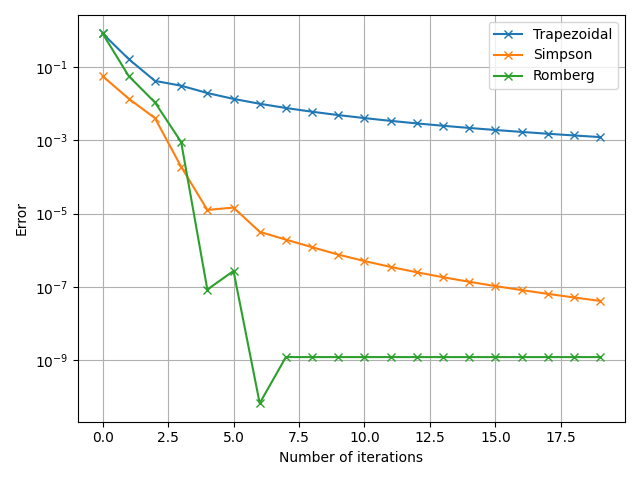
\includegraphics[width=0.45\linewidth]{res/convergence.png}
	\caption{Comparison of three different integration methods on $f(x) = \frac{1}{1 + x^2}$ over $[-1, 2]$.}
	\label{fig:convergence}
\end{figure}

\vspace*{-0.5cm}
